\subsection{Definition}
\begin{frame}{Popularity: Definition}
Since we are using MAL database and it has a social component, seems logic to use \emph{member\_favorites} as a representation of \emph{popularity}. We can also get popularity and score of anime from opinions of the same set of users.
\vspace{-10pt}

\begin{table}[!h]
	\begin{center}
	\begin{tabular}{|l|c|l|}
		\hline
		Name & Popularity & Some popular roles of them\\ 
		\hline
		Kana Hanazawa & 56637 & \textit{Angel Beats!}: Tachibana, Kanade \\
		\hline
		Hiroshi Kamiya & 49685 & \textit{Shingeki no Kyojin}: Levi, \\
		\hline
		Mamoru Miyano & 43942 & \textit{Death Note}: Yagami, Light \\ 
		\hline
		Rie Kugimiya & 31668 & \textit{Fullmetal Alchemist}: Elric, Alphonse \\ 
		\hline
		Jun Fukuyama & 26811 & \textit{Ao no Exorcist}: Okumura, Yukio \\ 
		\hline
		Miyuki Sawashiro & 26501 & \textit{Durarara!!}: Sturluson, Celty \\ 
		\hline
		Tomokazu Sugita & 24449 & \textit{Gintama}: Sakata, Gintoki \\
		\hline
		Daisuke Ono & 24080 & \textit{Durarara!!}: Heiwajima, Shizuo \\
		\hline
		Saori Hayami & 18322 & \textit{Owari no Seraph}: Hiiragi, Shinoa \\ 
		\hline
		Aya Hirano & 18094 & \textit{Fairy Tail}: Heartfilia, Lucy \\
		\hline
	\end{tabular}
	\end{center}
\end{table}
\end{frame}
%-------------------------------------------------------------------------

\subsection{Analysis}
\begin{frame}{Popularity: Analysis}
\begin{center}
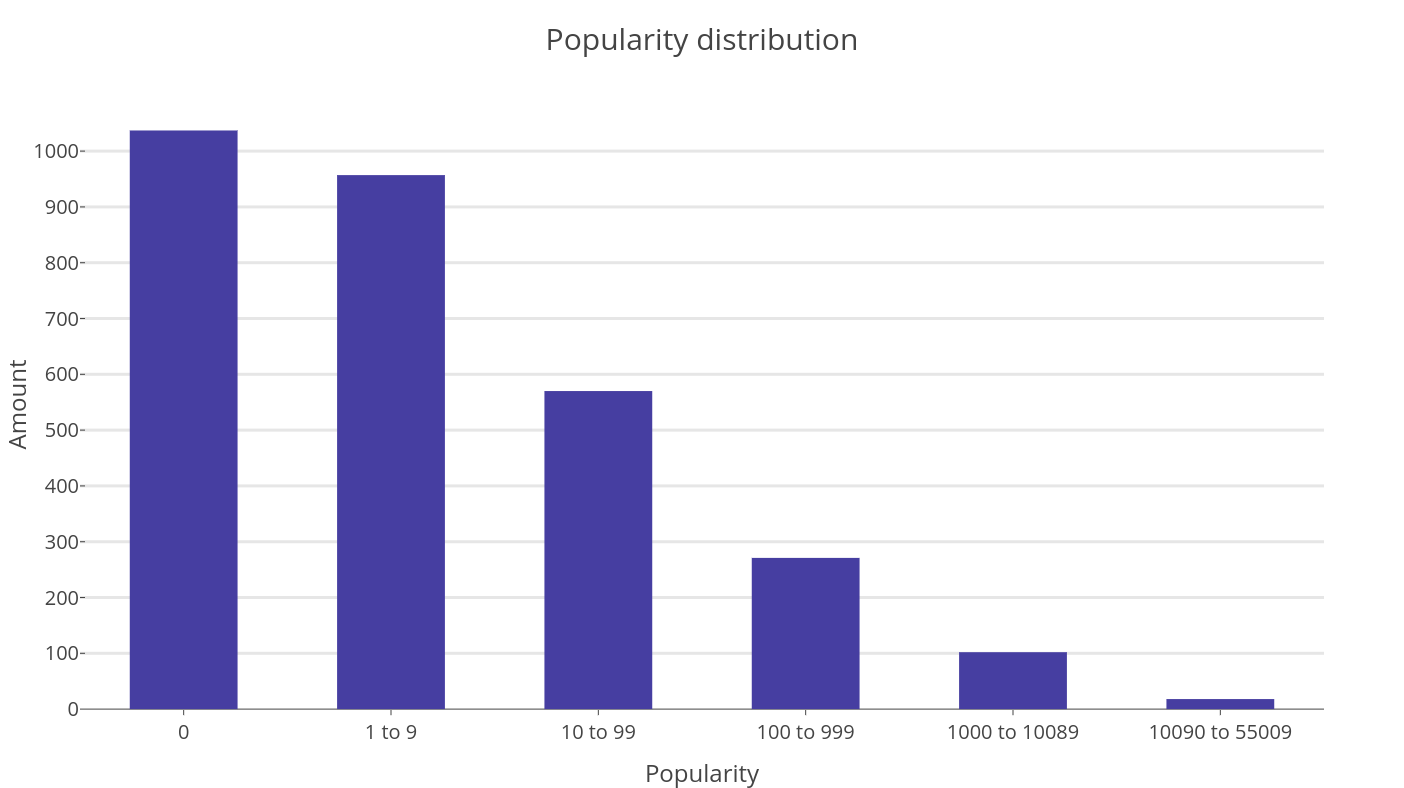
\includegraphics[scale=0.2]{graphics/popularityDistribution.png} 
\end{center}
\begin{table}[!htb]
    \begin{minipage}{.4\textwidth}
		\begin{itemize}
	\item Total: 2956
	\item Mean:    289.55
	\item Median:    2.0
		\end{itemize}
    \end{minipage}%
    \begin{minipage}{.6\textwidth}
        	\begin{itemize}
	\item Min:    0; Max:    55018
	\item 1037 values equal to zero
	\item Only 120 values bigger than 1000
		\end{itemize}
    \end{minipage}
\end{table}
\end{frame}
%-------------------------------------------------------------------------

\subsection{Pearson correlation}
\begin{frame}{Popularity: Pearson correlation}
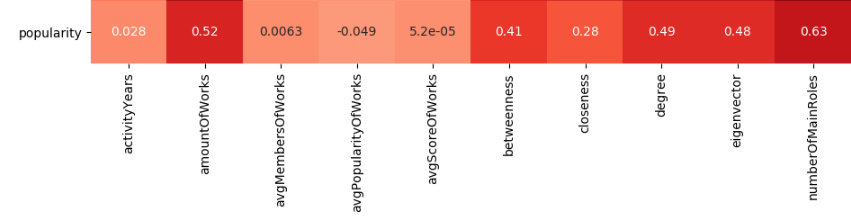
\includegraphics[scale=0.45]{graphics/popCorrelationAllWorks.png} 
\begin{itemize}
\item Big correlation between popularity and amount of works. %This attribute doesn't have the biggest correlation with popularity but "number of main roles" was added to the end of this investigation since we didn't had the data for doing so before. 
\item Number of main roles and amount of works have a strong correlation with each other (0.9) but they have different influence over popularity, this means they provide distinct information.
\end{itemize}

\end{frame}
%-------------------------------------------------------------------------

\begin{frame}
Since our dataset is biased in favor of more modern anime we thought of correlate with \emph{recent works} only.
\vspace{5pt}

But, how recent? Last 5, 10 or 20 years? 
\vspace{-5pt}

\begin{center}
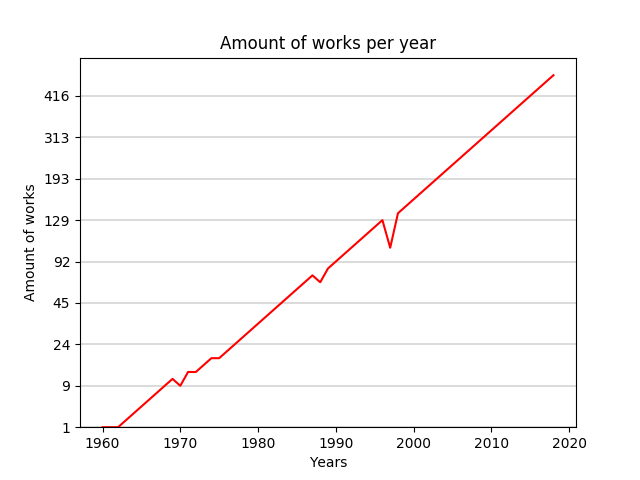
\includegraphics[scale=0.6]{graphics/worksPerYear_1960-2018.png} 
\end{center}

\end{frame}
%-------------------------------------------------------------------------

\begin{frame}
ENTONCES LA DEFINICION DE RECENT WORKS ES BLA
\begin{center}
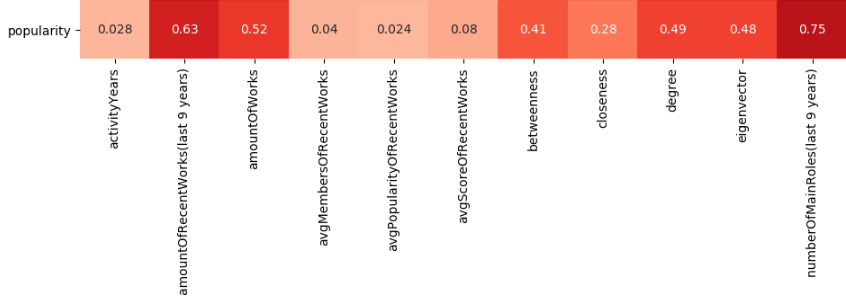
\includegraphics[scale=0.45]{graphics/popCorrelationRecentWorks.png} 
\end{center}
\begin{itemize}
\item TODO AGREGAR DATOS ACA COMO QUE RECENT WORKS ES MAS IMPORTANTE, BLA
\end{itemize}
\end{frame}
%-------------------------------------------------------------------------

\begin{frame}
EL HECHO DE QUE TRATAMOS DE EXPLICAR POR QUE? O MEJOR NO?
\begin{figure}
	\centering
	\begin{subfigure}{.4\columnwidth}
		\centering
		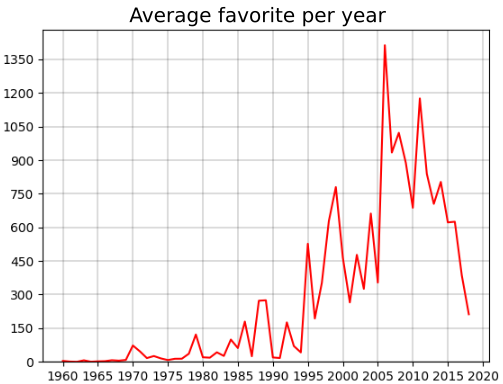
\includegraphics[width=\columnwidth]{graphics/avgFavorites.png}
	\end{subfigure}%
	\begin{subfigure}{.4\columnwidth}
		\centering
		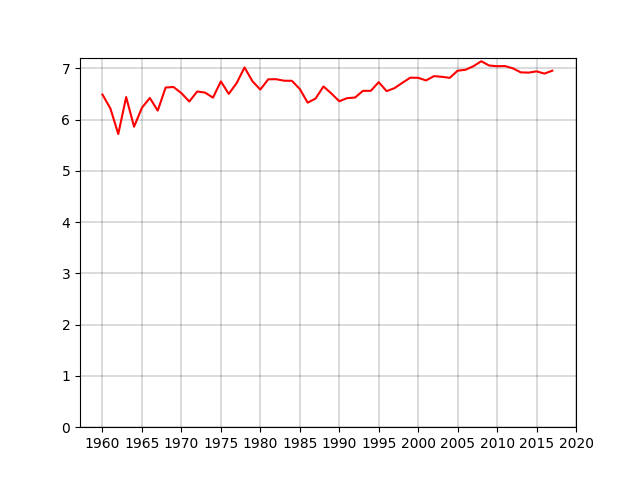
\includegraphics[width=\columnwidth]{graphics/avgScores.png}
	\end{subfigure}
	\begin{subfigure}{.4\columnwidth}
		\centering
		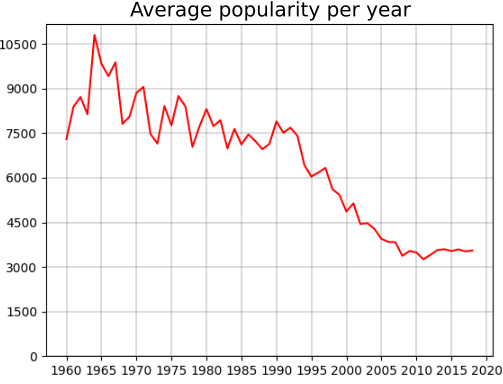
\includegraphics[width=\columnwidth]{graphics/avgPopularities.png}
	\end{subfigure}%
	\begin{subfigure}{.4\columnwidth}
		\centering
		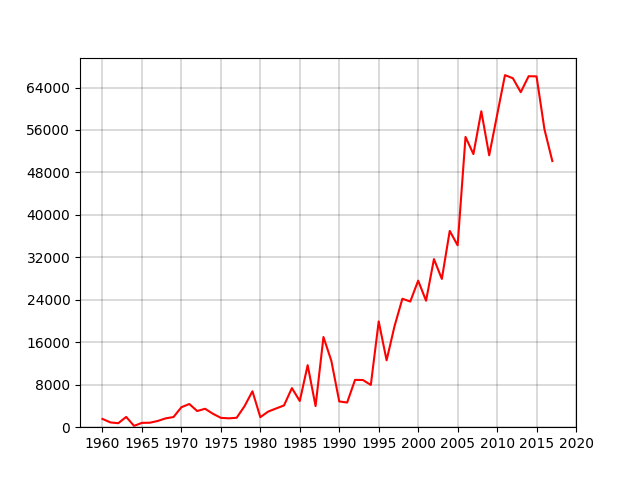
\includegraphics[width=\columnwidth]{graphics/avgMembers.png}
	\end{subfigure}
	\caption{Averages of favorites, score, popularity and amount of members.}
\end{figure}
\end{frame}
%-------------------------------------------------------------------------

\subsection{Prediction}
\begin{frame}
popularity
\end{frame}